\documentclass{article}
\usepackage{geometry}
\geometry{a4paper, margin=1in}
\usepackage{amsmath}
\usepackage{graphicx}
\usepackage{hyperref}
\usepackage{booktabs}
% Make czech characters work
\usepackage[czech]{babel}
%add package for python code
\usepackage{listings}
\usepackage{color}
\usepackage{float}
\usepackage{subcaption}
\usepackage{tikz}
\usepackage{pgfplots}
\usepackage{pgfplotstable}
\usepackage{filecontents}

\pgfplotsset{compat=1.18}

\lstset{
    language=Python,
    basicstyle=\ttfamily\small,
    keywordstyle=\color{blue},
    stringstyle=\color{red},
    commentstyle=\color{green},
    showstringspaces=false,
    numbers=left,
    numberstyle=\tiny\color{gray},
    breaklines=true,
    frame=single,
    inputencoding=utf8
}

\title{Brain excercise 6}
\author{Tomáš Jelínek}
\date{\today}

\begin{document}

\maketitle

\section*{Odpověď}

Zde je newick pro \textbf{UPGMA} strom:

((((F:0.05000,E:0.05000)Inner1:0.10000,D:0.15000)Inner2:0.03000,C:0.18000)

Inner4:0.10500,(B:0.15000,A:0.15000)Inner3:0.13500)Inner5:0.00000;

\begin{figure}[H]
    \centering
    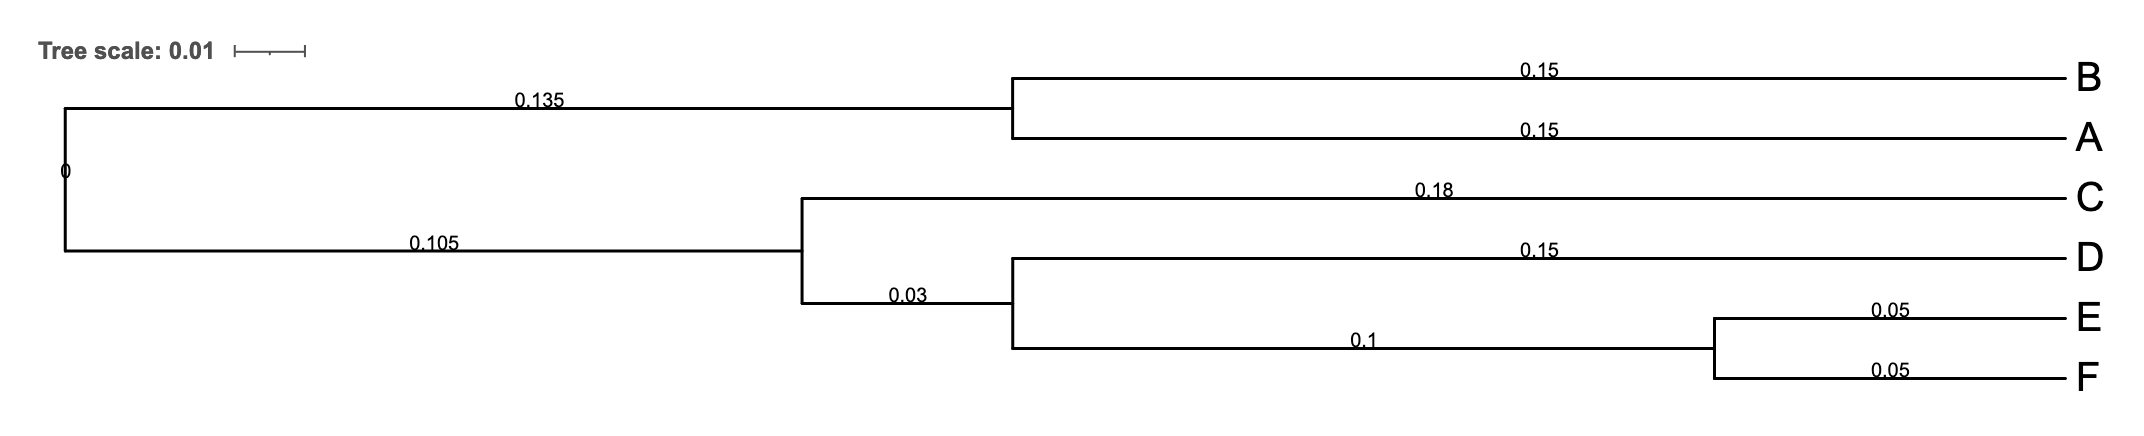
\includegraphics[width=0.8\textwidth]{upgma.png}
    \caption{UPGMA strom}
    \label{fig:upgma}    
\end{figure}

Zde je newick pro \textbf{Neighbor Joining} strom:

(((A:0.20000,B:0.10000)Inner1:0.24000,C:0.18000)Inner3:0.03000,D:0.15000,

(F:0.05000,E:0.05000)Inner2:0.10000)Inner4:0.00000;

\begin{figure}[H]
    \centering
    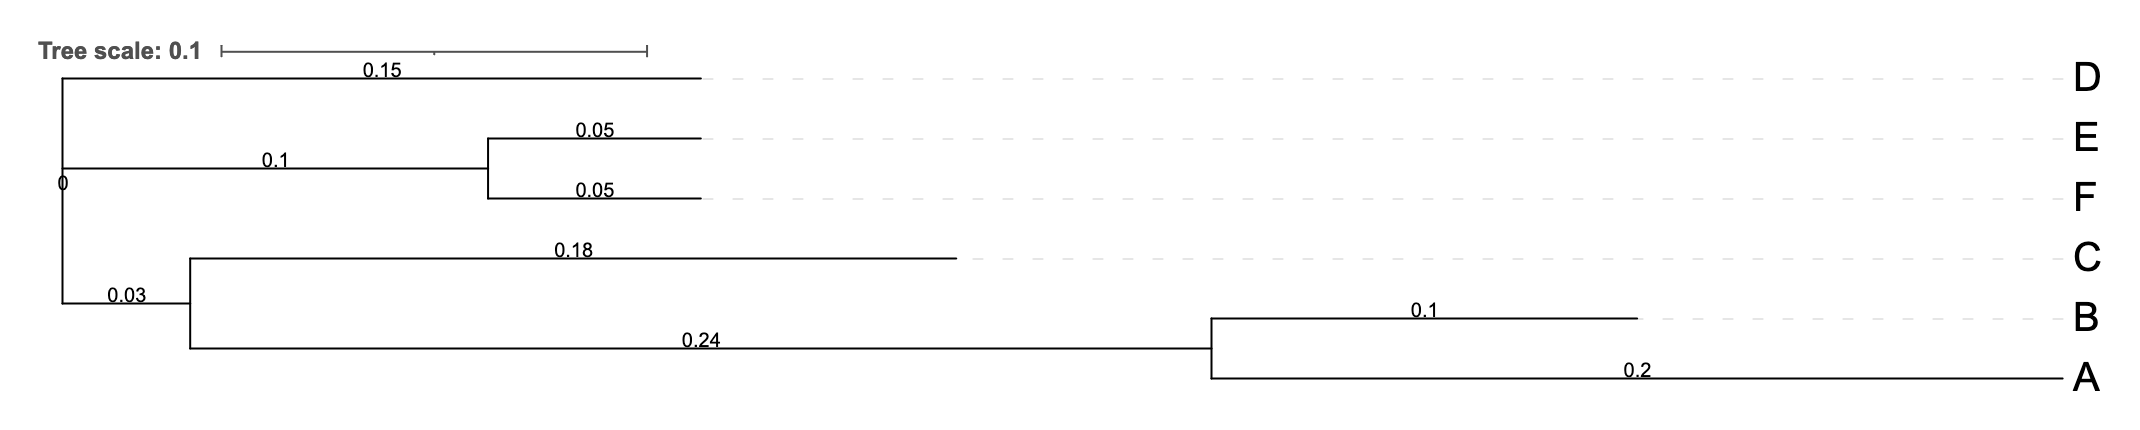
\includegraphics[width=0.8\textwidth]{nj.png}
    \caption{Neighbor Joining strom}
    \label{fig:nj}
\end{figure}

Z tohoto lze odečíst, že nejvyšší rychlost evoluce (substituční) má \textit{A} a i pak případně \textit{B}.

\subsection*{Python kód}

1.
\lstinputlisting[language=Python, inputencoding=utf8]{upgma.py}

2.
\lstinputlisting[language=Python, inputencoding=utf8]{test_upgma.py}


\end{document}
